\subsection{Edmonds-Karp}

\begin{algorithm}
  \caption{Algoritmo de Ford-Fulkerson}
  \begin{algorithmic}
    \Function{Ford-Fulkerson}{$network\ N$}
    \State Sea $F$ un flujo nulo
    \While{$\exists \text{ un camino dirigido de $s$ a $t$ sin lados saturados}$} 
    \State Sea $x_0, \mathellipsis, x_r$ un camino dirigido de $s$ a $t$
    \State $\varepsilon = \min_{0 \le i < r} \{C(\ora{x_i x_{i+1}}) - F(\ora{x_i x_{i+1}})\}$
    \State Mandar $\varepsilon$ unidades de flujo por el camino
    \EndWhile
    \EndFunction
  \end{algorithmic}
\end{algorithm}

\begin{definition}[Camino aumentante]
Sea $N = (V,E,C)$ un network y $F$ un flujo de $s$ a $t$, definimos a un \emph{camino $\boldsymbol{F}$-aumentante} como una sucesión de vértices $\{x_0,\mathellipsis, x_r\}$ tales que: $\forall i: 0 \le i < r :$
\begin{itemize}
    \item
    $x_{i+1} \in \Gamma^{+}(x_i) \equiv \ora{x_i x_{i+1}} \in E$ (es lado "\emph{forward}") si $F(\ora{x_i x_{i+1}}) < C(\ora{x_i x_{i+1}})$ (se puede enviar aún más flujo)
    \item
    $x_{i+1} \in \Gamma^{-}(x_i) \equiv \ora{x_{i+1} x_i} \in E$ (es lado "\emph{backward}") si $F(\ora{x_{i+1} x_i}) > 0$ (se puede devolver flujo)
\end{itemize}
\end{definition}

\begin{definition}[Flujo en un camino aumentante]
Sea $N$ un network, $F$ un flujo, y $\{x_0,\mathellipsis,x_r\}$ un camino $F$-aumentante entre $s$ y $t$. Enviar $\varepsilon$ unidades de flujo a través de ese camino consiste en:\\
Definir una función $F^* \colon E \to \mathbb{R}_{\ge 0}$ tal que:
\begin{align}
    F^*(\ora{xy}) &= F(\ora{xy}) &\text{ si $\ora{xy}$ no está en el camino aumentante} \\
    F^*(\ora{x_i x_{i+1}}) &= F(\ora{x_i x_{i+1}}) + \varepsilon & x_{i+1} \in \Gamma^{+}(x_i) \\
    F^*(\ora{x_i x_{i+1}}) &= F(\ora{x_i x_{i+1}}) - \varepsilon & x_{i+1} \in \Gamma^{-}(x_i)
\end{align}
\end{definition}

\begin{lemma}\label{flujo_camino_aumentante}
Sea $F$ un flujo en un network $N$ entre $s$ y $t$ y sea $\{x_0,\mathellipsis,x_r\}$ un camino $F$-aumentante.\\
Definimos $\forall i: 0\le i < r:$  \begin{align}
    \varepsilon_i = \left\{
    \begin{array}{cc}
         C(\ora{x_i x_{i+1}}) - F(\ora{x_i x_{i+1}}) &\text{ si } x_{i+1} \in \Gamma^{+}(x_i)\\
         F(\ora{x_{i+1} x_i}) &\text{ si } x_{i+1} \in \Gamma^{-} (x_i)
    \end{array}
    \right.
\end{align}
y $\varepsilon = min\{\varepsilon_i\mid 0\le i < r \}$.\\

Entonces, al enviar $\varepsilon$ unidades de flujo por el camino $F$-aumentante obtenemos un nuevo flujo $F^{*}$ y \begin{align}
    v_{F^{*}} = v_F + \varepsilon
\end{align}
\end{lemma}

\begin{proof}
Probaremos \textit{feasibility} y conservación:\\
\textit{Feasibility}: 
\begin{enumerate} 
\item $0 \le F^{*}(\ora{xy})$ siempre que $F(\ora{xy}) \le F^{*}(\ora{xy})$. (caso forward)\\
Cuando esto no pasa,  $F^{*}(\ora{x_{i+1} x_i}) = F(\ora{x_{i+1} x_i}) - \varepsilon \ge 0$ pues $\varepsilon \le \varepsilon_{i} = F(\ora{x_{i+1} x_i})$ (caso backward)
\item $F^{*}(\ora{xy}) \le C(\ora{xy})$ se cumple siempre que $F^{*}(\ora{xy}) \le F(\ora{xy}) \le C(\ora{xy})$. (caso backward) \\
Si no, $F^*(\ora{x_i x_{i+1}}) = F(\ora{x_i x_{i+1}}) + \varepsilon \le F(\ora{x_i x_{i+1}}) + C(\ora{x_i x_{i+1}})- F(\ora{x_i x_{i+1}}) \le C(\ora{x_i x_{i+1}})$.  (caso forward)
\end{enumerate}
Conservación:
Si $x$ no pertenece al camino, no pasa nada.\\
Sea $x= x_i \neq s, t$. Es decir, $i \neq 0, r$\\

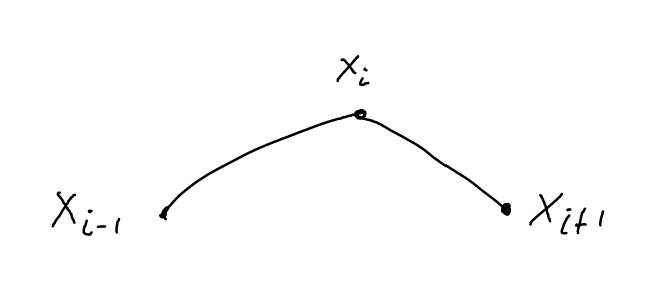
\includegraphics[scale=0.4]{img/base.png}\\
Hay 4 casos posibles:
\begin{enumerate}

\item $x_{i+1} \in \Gamma^+(x_i)$ y $x_i\in \Gamma^+(x_{i-1})$: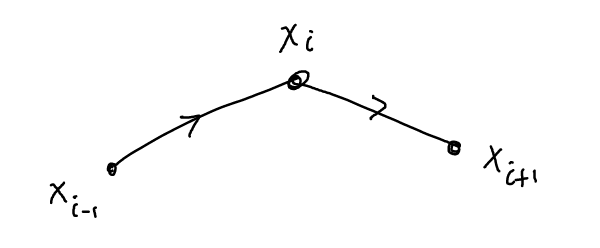
\includegraphics[scale=0.4]{img/forward-forward.png}\\
Como 
\begin{align}
    \left.
    \begin{array}{cc}
    F^*(\ora{x_i x_{i+1}}) = F(\ora{x_i x_{i+1}}) + \varepsilon\\
    F^*(\ora{x_{i-1} x_i}) = F(\ora{x_{i-1} x_i}) + \varepsilon 
    \end{array}
     \right\} \implies
     \begin{array}{cc}
    out_{F^*}(x_i) = out_F(x_i) + \varepsilon \\
    in_{F*} (x_i) = in_F(x_i) + \varepsilon
    \end{array}
\end{align}
$\therefore out_{F^*} (x_i) - in_{F^*}(x_i) = 0.$\\
Cambiaron los lados que entran y salen de $x_i$.
    
\item $x_{i+1} \in \Gamma^+(x_i)$ y $x_{i-1} \in \Gamma^{-}(x_{i})$: 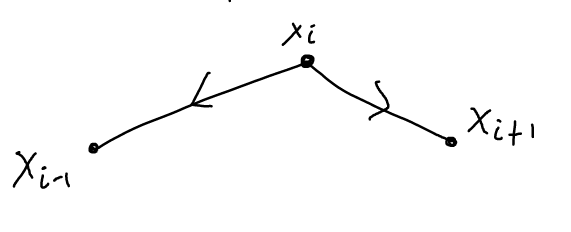
\includegraphics[scale=0.4]{img/backward-forward.png}\\
\begin{align}
    \left.
    \begin{array}{cc}
    F^*(\ora{x_i x_{i+1}}) = F(\ora{x_i x_{i+1}}) + \varepsilon\\
    F^*(\ora{x_{i-1} x_i}) = F(\ora{x_i x_{i+1}}) - \varepsilon 
    \end{array}
     \right\} \implies
     \begin{array}{cc}
    out_{F^*}(x_i) = out_F(x_i) + \varepsilon -  \varepsilon = out_F(x_i)\\
    in_{F^*} (x_i) = in_F(x_i)
    \end{array}
\end{align}
$\therefore out_{F^*} (x_i) - in_{F^*}(x_i) = 0.$\\
Cambiaron dos lados que salen de $x_i$ y ninguno que entra a $x_i$ cambió.

\item $x_i \in \Gamma^-(x_{i+1})$ y $x_i\in \Gamma^+(x_{i-1}):$ 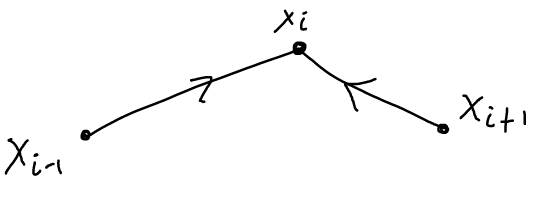
\includegraphics[scale=0.4]{img/forward-backward.png}\\
\begin{align}
    \left.
    \begin{array}{cc}
    F^*(\ora{x_{i+1} x_i}) = F(\ora{x_{i+1} x_i}) - \varepsilon\\
    F^*(\ora{x_{i-1} x_i}) = F(\ora{x_{i-1} x_i}) + \varepsilon 
    \end{array}
     \right\} \implies
     \begin{array}{cc}
    out_{F^*}(x_i) = out_F(x_i) + \varepsilon -  \varepsilon = out_F(x_i)\\
    in_{F^*} (x_i) = in_F(x_i)
    \end{array}
\end{align}

\item $x_{i}\in \Gamma^-(x_{i+1})$ y $x_{i-1} \in \Gamma^-(x_{i})$: 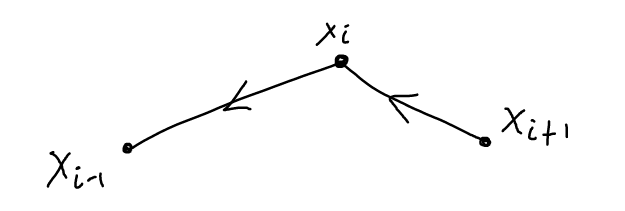
\includegraphics[scale=0.4]{img/backward-backward.png}
\begin{align}
    \left.
    \begin{array}{cc}
    F^*(\ora{x_i x_{i-1}}) = F(\ora{x_{i} x_{i-1}}) - \varepsilon\\
    F^*(\ora{x_{i+1} x_{i}}) = F(\ora{x_{i+1} x_{i}}) - \varepsilon 
    \end{array}
     \right\} \implies
     \begin{array}{cc}
    out_{F^*}(x_i) = out_F(x_i) + \varepsilon -  \varepsilon = out_F(x_i)\\
    in_{F^*} (x_i) = in_F(x_i)
    \end{array}
\end{align}

\end{enumerate}

Respecto al $v_{F^*}$ tenemos que:\\
Si $x_1 \in \Gamma^+(s)$ entonces
\begin{align}
    V_{F*} &= out_{F^*}(s) - in_{F^*}(s)\\
        &= out_F(s) + \varepsilon - in_{F}(s)\\
        &= v_F + \varepsilon
\end{align}
Si $x_1 \in \Gamma^-(s)$ entonces
\begin{align}
    v_{F^*} &= out_{F^{*}}(s) - in_{F^*}(s)\\
        &= out_F(s) - (in_F(s) - \varepsilon)\\
        &= v_F + \varepsilon
\end{align}
\end{proof}

\begin{lemma}
Sea $N$ un network, $G$ un flujo de $s$ a $t$ y $S$ un corte cualquiera, entonces
\begin{align}
    v_G = G(S, S^c) - G(S^c, S)
\end{align}
\end{lemma}

\begin{proof}
Sea $x\in S$. Vemos que $out_G(x) - in_G(x) = \left\{
    \begin{array}{cc}
     0  &x\neq s\\
     v_G &x = s
    \end{array}
\right.$\\

\begin{align}
    \therefore v_G &= \sum_{x\in S} out(x) - in(x) = \sum_{\substack{x\in S\\xv \in E}} G(x,v) - G(v,x)\\
    &= G(S,V) - G(V,S)  &&\text{Aca usamos: } S \cup S^c = V \wedge S \cap S^c = \varnothing \\
    &= G(S,S) + G(S, S^c) - G(S,S) - G(S^c, S)\\
    &= G(S,S^c) - G(S^c, S)
\end{align}

\end{proof}

\begin{corollary}
El valor del flujo es una cota inferior de la capacidad de un corte $S$ esto es: $v_G \le cap(S)$
\end{corollary}
\begin{proof}
Por restricción de capacidad y conservación, sabemos que \\$G(S, S^c) \le C(S, S^c)$ y $G(S^c, S) \ge 0$ entonces vale:
\begin{align}
v_G &= G(S, S^c) - G(S^c, S)\\
	&\le G(S, S^c)\\
    &\le cap(S)
\end{align}
\end{proof}

\begin{theorem}[\textit{Max-flow min-cut}]
Sea $N = (V,E,C)$ un network, $F$ un flujo de $s$ a $t$ en $N$ y $S$ un corte minimal de $V$ entonces
\begin{align}
    \underbrace{F \text{ es maximal}}_{A} \iff 
    \underbrace{\nexists \text{ caminos } F\text{-aumentantes entre $s$ y $t$}}_{B} \iff
    \underbrace{v_F = mincutcap_S}_{C}
\end{align}
\end{theorem}
\begin{proof}
$C \implies A:$\\
Asumamos $C)$. Sea $S$ un corte con $cap(S) = v_F$\\
Sea $G$ otro flujo. Tenemos por [ref] que
\begin{align} v_G \le cap(S) = v_F \end{align}
de lo que se sigue que $F$ es maximal.\\

Notar que así mismo, $S$ es minimal pues dado un corte cualquiera $T$\begin{align}
    cap(T) \ge v_F = cap(S)
\end{align}
$B \implies C:$\\
Sea $S = \{s\} \cup \{x \in V \mid \exists \text{ camino $F$-aumentante de $s$ a $x$}$\}.
Es claro que $t \notin S$ pues por hipótesis \\$\nexists$ caminos $F$-aumentantes de $s$ a $t$.\\
$\therefore S$ es corte.\\
Como $S$ es corte,
\begin{align}
    v_F = F(S, S^c) - F(S^c, S)
\end{align}
Sea $x \in S$, $y \in S^c$, $\ora{xy} \in E$. Buscamos $F(xy)$, y vemos que:
\begin{itemize}
    \item $\exists$ un camino F-aumentante $(x_0, x_1,\mathellipsis, x_r)$ entre $s$ y $x$
    \item $\nexists$ un camino $F$-aumentante entre $s$ e $y$
\end{itemize}
Esto es, $(x_0, \mathellipsis, x_r, y)$ no es un camino $F$-aumentante.\\
Como $(x_0, x_1, \mathellipsis, x_r)$ si lo es, y $\ora{xy} \in E$, concluimos que $\ora{xy}$ está saturado, ie. \\$F(\ora{xy}) = C(\ora{xy})$.
\begin{align}
    \therefore \forall x,y: x \in S \wedge y \in S^c \wedge xy \in E : F(\ora{xy}) = C(\ora{xy})\\
    F(S, S^c) = \sum_{\substack{x\in S\\ y \notin S \\\ora{xy} \in E}} F(\ora{xy}) = \sum_{\substack{x\in S\\ y \notin S\\ \ora{xy} \in E}} C(\ora{xy}) = C(S, S^c) = cap(S)\\
\end{align}
Ahora, veamos el otro caso. Sea $x \in S^c, y \in S, \ora{xy} \in E$. Buscamos $F(\ora{xy})$. Con un análisis similar al anterior, teniendo en cuenta que ahora $x\in \Gamma^-(y)$, concluimos $xy$ está vacio ie. $F(\ora{xy}) = 0$.
\begin{align}
    \therefore \forall x, y : x \in S^c \wedge y \in S \wedge xy \in E : F(\ora{xy}) = 0\\
    F(S^c, S) = \sum_{\substack{x\not\in S\\ y \in S\\ \ora{xy} \in E}} F(\ora{xy}) = \sum_{\substack{x\not\in S\\ y \in S\\ \ora{xy} \in E}} 0 = 0
\end{align}
Así,
\begin{align}
v_F = F(S, S^c) - F(S^c, S) = cap(S) - 0 = cap(S) = mincutcap_S
\end{align}
Por último, $S$ es claramente minimal.

$A \implies B$:\\
Suponiendo $F$ maximal, supongamos que $B$ es falso, es decir, que existe un camino $F$-aumentante entre $s$ y $t$.\\
Por el lema [\ref{flujo_camino_aumentante}], es posible enviar $\varepsilon$ unidades de flujo por ese camino y obtener un flujo $F^*$ con $v_{F^*} = v_F + \varepsilon$. Esto es absurdo pues $F$ es maximal.
\end{proof}

\begin{algorithm}
\caption{Algoritmo de Edmonds-Karp para hallar flujo maximal}
\begin{algorithmic}
\Require network $N=(V,E,C)$
\Ensure  $(F, v, S)$ donde $F$ es flujo maximal, $v$ es el valor del flujo y $S$ es el corte minimal
\Function{Edmonds-Karp}{$network\ N$}
\State $F = 0, v = 0, \varepsilon(s) = \infty$
\While{$true$} 
    \State $queue\ Q = qEmpty()$
    \State $qEnqueue(Q,s)$
    \State $S := \{s\}$
    \While{$qCnt(Q)$}
        \State $x = qDequeue(Q)$
        \State \ForAll{$z \in \Gamma^{+}(x) \cap S^c$}
        \If{$F(xz) < C(xz)$}
            \State $qEnqueue(Q,z)$
            \State $S = S \cup \{z\}$
            \State $a(z) = x;\ b(z) = 1$
            \State $\varepsilon(z) = min\{\varepsilon(x), C(xz) - F(xz)\}$
        \EndIf
        \EndFor
        \State \ForAll{$z\in \Gamma^{-}(x) \cap S^c$}
        \If{$F(zx) > 0$}
        \State $qEnqueue(Q,z)$
        \State $S = S \cup \{z\}$
        \State $a(z) = x;\ b(z) = -1$
        \State $\varepsilon(z) = min\{\varepsilon(x), F(zx)\}$
        \EndIf
        \EndFor
        \EndWhile
        \State
        \If{$t \in S$}
        \State $q = t;\ \varepsilon = \varepsilon(t);\ v = v+E$
        \While{$q \neq s$}
        \State $p = a(q)$
        \If{$b(q) == 1$}
        \State $F(pq) = F(pq) + \varepsilon$
        \State $F(qp) = F(qp) - \varepsilon$
        \EndIf
        \State q = p;
        \EndWhile
        \Else
        \State \Return{$F, v, S$}
        \EndIf
\EndWhile
\EndFunction
\end{algorithmic}
\end{algorithm}

\begin{theorem}[Teorema de integralidad]\label{integrality}
Sea $N=(V,E,C)$ un network tal que $\forall xy \in E : C(xy) \in \mathbb{Z}$ entonces $\exists$ flujo maximal entero.

En otras palabras, en un network con capacidades enteras encontraremos siempre un flujo maximal entero.
\end{theorem}

\begin{proof}
Lo probaremos por inducción, corriendo el algoritmo de Ford-Fulkerson en $n+1$ pasos, sean $F_0, \mathellipsis, F_n$ los sucesivos flujos obtenidos:\\
Caso base: $F_0 = 0 \in \mathbb{Z}$.\\
Caso inductivo:
$F_k \in \mathbb{Z} \implies F_{k+1} \in \mathbb{Z}$\\
$F_{k+1}$ se construye a partir de $F_k$, cambiando en algunos lados el valor $F_k$ por $F_k \pm \varepsilon$. Por lo tanto, si probamos que $\varepsilon \in \mathbb{Z}$, también tendremos que $F_{k+1} \in \mathbb{Z}$. Luego,
\begin{align}
    \varepsilon = \min\{\epsilon_i\}
\end{align}
y \begin{center}
    $\epsilon_i = \begin{cases} C(\ora{x_i x_{i+1}}) - F(\ora{x_i x_{i+1}}) & \text{ si } \ora{x_i x_{i+1}} \text{ es lado forward}\\
    F(\ora{x_{i+1} x_i}) & \text{ si } \ora{x_i x_{i+1}} \text{ es lado backward}
    \end{cases}$
\end{center}
Como las capacidades son todas enteras, $\epsilon_i$ es entero, $\varepsilon$  es entero y por lo tanto $F_{k+1}$.
Esto prueba que si Ford-Fulkerson termina, obtenemos un flujo maximal entero.
Como $v_{F_{k+1}} - v_{F_k} = \varepsilon \in \mathbb{Z} > 0$, por lo tanto $\varepsilon \ge 1$. Esto es, el ``salto" que se produce entre un flujo y el siguiente es discreto.
Como existe una cota superior para el conjunto de valores de flujos posibles (por ej. $cap(S)$), esta sucesión de flujos debe ser finita. 
\end{proof}

\begin{definition}
Dados $a,b\in V$ y un flujo $F$ en un network $N = (V,E,C)$. Definimos a la \emph{distancia (respecto de $\boldsymbol{F}$) de $\boldsymbol{a}$ hasta $\boldsymbol{b}$} como:
\begin{align}
D_F(a,b) = \left\{
    \begin{array}{cc}
         0 & a = b\\
         \#\{x_i x_{i+1} \in E\mid 0\le i < r \}  &\text{si $\{x_0, \mathellipsis, x_r\}$ es el menor camino $F$-aumentante entre $a$ y $b$} \\ 
         \infty &\text{si $\nexists$ camino $F$-aumentante entre $a$ y $b$}
    \end{array}
    \right.
\end{align}
Esto es, el numero de lados del menor camino aumentante relativo a $F$ entre $a$ y $b$.\\
Asimismo, definimos
\begin{itemize}
    \item $d_F(x) \doteq D_F(s,x)$
    \item $b_F(x) \doteq D_F(x,t)$
\end{itemize}
\end{definition}

\begin{lemma}\label{distancias_no_decrecen_EK}
Sea $N=(V,E,C)$ un network y $F_1, F_2, \mathellipsis, F_\ell$ los flujos parciales obtenidos por Edmonds-Karp (supongamos que $F_0 = 0$ es el flujo inicial).\\
Abreviaremos
\begin{align}
    d_k(x) \doteq d_{F_k}(x) \\
    b_k(x) \doteq d_{F_k}(x)
\end{align} entonces tenemos que $\forall x \in V$:
\begin{align}
    d_k(x) \le d_{k+1}(x) \\
    b_k(x) \le b_{k+1}(x)
\end{align}
\end{lemma}

\begin{proof}
$\forall i : 1 \le i \le \ell$ :\\
\begin{enumerate}
    \item
    Sea $A_i \doteq \{x \in V \mid d_i(x) < d_{i-1}(x)\}$, queremos ver que $A_i = \varnothing$ comenzando por notar que $s \notin A_i$ ya que $\forall i: d_i(s) = 0$.\\
    Supongamos que $\exists i : A_i \neq \varnothing$. Sea ese $i$ el mínimo posible. A su vez, sea $x = \min\{d_i(v) \mid v \in A_i \}$, ie. tal que $d_i(x)$ sea mínimo. Entonces, $\forall z : d_i(z) > d_i(x) \implies z\notin A_i$.\\
    Como $d_i(x) < d_{i-1}(x) \le \infty$ tenemos que $d_i(x) < \infty$ y debe haber un camino $F_i$-aumentante de $s$ a $x$. Sea $(x_0, \mathellipsis, x_r)$ el camino mínimo (es decir, con $r = d_i(x)$).\\
    Probemos ahora que $\nexists$ un camino $F_{i-1}$-aumentante de $s$ a $x$, y luego lleguemos a una contradicción.\\
    Sea $z = x_{r-1}$. Como $(x_0,\mathellipsis, x_r)$ es el camino $F_i$-aumentante de menor longitud entre $s$ y $x$ entonces $(x_0, \mathellipsis, x_{r-1})$ es el camino $F_{i}$-aumentante de menor longitud entre $s$ y $z$. Así, como $d_i(z) = r-1$ se sigue que $z \notin A_i$. Concluimos que $d_{i-1}(z) \le d_i(z) < d_i(x) < d_{i-1}(x)$. \\
    $\therefore d_{i-1}(z) \le d_{i-1}(x)-2$.
    Pero consideremos que $d_{i-1}(x) \le d_{i-1}(z) + 1$, ya que se puede ir de $z$ a $x$.
    Como $d_{i-1}(z)+2 \le d_{i-1}(x)$, esto es absurdo.\\
    $\therefore \nexists$ camino $F_{i-1}$-aumentante $(s,\mathellipsis, z, x).$\\
    Ahora la contradicción:\\
    Como existe un camino $(s, \mathellipsis, z, x)$, debe pasar $x \in \Gamma^+(z)$ o bien $x \in \Gamma^-(z)$. La razón por la que no existe un camino $F_{i-1}$ aumentante puede ser alguna de las siguientes:
    \begin{itemize}
        \item $x \in \Gamma^+(z) \wedge F_{i-1}(\ora{zx}) = C(\ora{zx})$
        \item $x \in \Gamma^-(z) \wedge F_{i-1}(\ora{zx}) = 0$ 
    \end{itemize}
    Pero como el camino $F_i$-aumentante si existe,
    \begin{itemize}
        \item $x \in \Gamma^+(z) \wedge F_{i-1}(\ora{zx}) = C(\ora{zx}) \wedge F_i(\ora{zx}) < C(\ora{zx})$
        \item $x \in \Gamma^-(z) \wedge F_{i-1}(\ora{zx}) = 0 \wedge F_i(\ora{zx}) > 0$
    \end{itemize}

    La única forma en que esto puede ocurrir es que al pasar de $F_{i-1}$ a $F_i$ usemos un camino de la forma $(s, \mathellipsis, x, z)$, ya que:
    \begin{itemize}
        \item Si el último lado es backward, $x \in \Gamma^+(z) \wedge F_{i}(\ora{zx}) < F_{i-1}(\ora{zx})$ (primer razón).
        \item Si el último lado es forward, $x \in \Gamma^-(z) \wedge F_{i}(\ora{xz}) > F_{i-1}(\ora{xz})$ (segunda razón).
    \end{itemize}
    Como usamos Edmonds-Karp, este camino tiene longitud mínima.
    Entonces $d_{i-1}(z) = d_{i-1}(x) + 1$. Pero sabemos que $d_{i-1}(x) + 1  = d_{i-1}(z) \le d_{i-1}(x) - 2$. Esto es una contradicción. Concluimos:
    \begin{align}
        \nexists i : A_i \neq \varnothing
        \equiv
        \forall i : A_i = \varnothing
    \end{align}
    Es decir, $\forall i, x : x \in V : d_{i-1}(x) \le d_i(x)$
    \item
    Similarmente, podemos construir un $B_i = \{x \in V \mid b_i(x) < b_{i-1}(x) \wedge i \ge 1\}$ y probar que
    \begin{align}
    \forall i : B_i = \varnothing && \text{ie.}\\
    \forall i, x : x \in V : b_{i-1}(x) \le b_i(x)
    \end{align}
    \end{enumerate}
\end{proof}

\begin{theorem}[Complejidad del algoritmo de Edmonds-Karp] 
El algoritmo de Edmonds-Karp para encontrar un flujo maximal y un corte minimal en un network es de complejidad $\mathcal{O}(n m^2)$
\end{theorem}
\begin{proof}
Notemos que al construir cada $F_i$ pasa una de las siguientes:
\begin{itemize}
    \item Al menos un lado forward se satura.
    \item Al menos un lado backward se vacía.
\end{itemize}
Llamamos \emph{crítico} a un tal lado.
Supongamos que un lado con vértices $x$ y $z$ se volvió crítico en el paso $i$. Antes de que pueda volverse crítico deberá usarse para el otro lado (si se usó como forward, debe usarse como backward, y viceversa). Supongamos que sucede eso en el paso $j > i$.\\
Así, $(s, \mathellipsis, z, x)$ es un camino mínimo en el paso $i$, y $(s,\mathellipsis, x, z)$ en el paso $j$.
Como el camino $F$-aumentante de $s$ a $t$ en el paso $j$ contiene a $z$:
\begin{align}
    d_j(t) = d_j(z)+b_j(z)
    \end{align}
Además, $z$ está después de $x$ en este camino:
\begin{align}
    d_j(t) = d_j(x) + 1 + b_j(z)
\end{align}
Por el lema [\ref{distancias_no_decrecen_EK}], sabemos que $d_{i-1}(x) \le d_i(x)$ (haciendo la sustitución: $i-1 := i \wedge i := j$) y:\begin{align}
    d_j(t) \ge d_i(x) + 1 + b_i(z)
\end{align}
Y ahora, en el paso $i$, $z$ está antes que $x$:
\begin{align}
    d_j(t) \ge d_i(x) + 1 + 1 + b_i(x)
\end{align}
Y entonces:
\begin{align}
    d_j(t) \ge d_i(t) + 2
\end{align}
Concluimos que si un lado se vuelve crítico, antes de que pueda volver a hacerlo, la distancia entre $s$ y $t$ debe aumentar en al menos $2$.\\
Por lo tanto, un lado puede volverse crítico a lo sumo $\frac{n+1}{2} \in \mathcal{O}(n)$ veces.
Sabemos que en la construcción de cada $F_i$ al menos un lado se vuelve crítico. Así, tenemos que \begin{align}
    \# F_i &\le m * \# \text{veces que puede volverse crítico}\\
    \# F_i &\in \mathcal{O}(nm)
\end{align}
Cada corrida consiste en construir un $F_i$ mediante $BFS \in \mathcal{O}(m)$.\\
 $\therefore$ La complejidad del algoritmo Edmonds-Karp es $\mathcal{O}(m) * \mathcal{O}(nm) = \mathcal{O}(nm^2)$
\end{proof}

